	
\section{Estructura de la aplicación}

La aplicación ha sido diseñada bajo la siguiente estructura:

\begin{itemize}	
	\item Vistas de usuario que son explicadas en la sección \ref{sec:vistasUsuario}.
	\item Scripts en lenguaje \textit{PHP} y \textit{Javascript} para dar soporte de comunicación de datos.
	\item Archivos ejecutables del aplicativo.
	\item Estructura de carpetas para dar persistencia a los datos de usuario.
\end{itemize} 

La aplicación se estructura de acuerdo a la figura \ref{fig:estruApp}.

\begin{figure}[H]
	\centering
	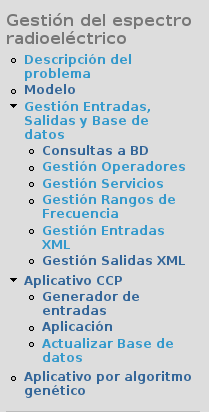
\includegraphics[width=3.5cm]{Capitulo8InterfacesWeb/Imagenes/AplicativoCPP.png}
	\caption{Estructura de aplicación}
	\label{fig:estruApp}	
\end{figure}

Como se observa en la anterior figura el aplicativo se divide en dos grandes partes: la primera que es la sección de gestión de la base de datos de gestión del espectro, donde se puede gestionar la información sobre el estado de las asignaciones o realizar y la segunda son los aplicativos que permiten encontrar soluciones y desplegar soluciones a instancias del problema.
\\\\
Para el uso de la aplicación se recomienda consultar los manuales de usuario en la página \pageref{sec:ManualesdeUsuario}

\subsection{Módulos de la aplicación}

La aplicación se encuentra organizada por módulos, cada uno de los cuales cumple una función específica. Estos módulos han sido diseñados de acuerdo a la especificación de estructura de la aplicación y para facilitar el uso a los usuarios finales.

\subsubsection{Gestión base de datos}

El módulo de gestión de base de datos presenta dos grandes funciones, la primera de ellas es la consulta de información a la base de datos y la segunda es de realizar operaciones de edición sobre parte de la información almacenada.
\\\\
En la tabla \ref{tabla:consultaApp} se explican las operaciones de consulta de información almacenada en la base de datos:

\begin{center}
\begin{longtable}{|p{7cm}|p{9cm}|}
	\caption{Consultas en el aplicativo prototipo de gestión del espectro} \label{tabla:consultaApp}\\
	\hline
	\cellcolor[gray]{0.9} \textbf{Consulta} & \cellcolor[gray]{0.9}\textbf{Descripción} \\
	\hline
	Consultar por entidad territorial por banda & Permite consultar en una zona geográfica determinada la asignación en una banda de frecuencia seleccionada.\\
	\hline
	Consultar por entidad territorial por operador & Despliega la información sobre la asignación en un territorio de un operador en específico.\\
	\hline
\end{longtable}	
\end{center}

En la tabla \ref{tabla:editarApp} se muestran las operaciones de edición de información que se encuentra en la base de datos:
\begin{center}
\begin{longtable}{|p{7cm}|p{9cm}|}
	\caption{Operaciones de edición en la base de datos gestión del espectro} \label{tabla:editarApp}\\
	\hline
	\cellcolor[gray]{0.9} \textbf{Operación} & \cellcolor[gray]{0.9}\textbf{Descripción} \\
	\hline
	Consultar por entidad territorial por banda & Permite consultar en una zona geográfica determinada la asignación en una banda de frecuencia seleccionada.\\
	\hline	
	Gestión Operadores & Permite agregar o editar operadores, no es posible eliminar un operador para garantizar integridad de los datos. También permite agregar o quitar servicios que presta un operador.\\
	\hline
	Gestión Servicios& Permite agregar o editar servicios, no es posible eliminar debido a la gran dependencia de los datos de asignaciones, operadores y rangos de frecuencia asociados a un servicio.\\
	\hline
	Gestión Rangos de Frecuencia & Permite editar o crear rangos de frecuencia, no es posible eliminar un rango de frecuencia para garantizar integridad de los datos. La creación de rangos de frecuencia permite especificar las formulas de transmisión o recepción de los canales, una vez creado un rango de frecuencia es posible editar sus canales individualmente.\\
	\hline
	Gestión Entradas XML& Permite visualizar, descargar y eliminar entradas XML que tenga el usuario almacenadas en el servidor.\\
	\hline	
	Gestión Salidas XML& Permite visualizar, descargar y eliminar salidas XML que tenga el usuario almacenadas en el servidor.\\
	\hline
\end{longtable}	
\end{center}

\subsubsection{Generador de entradas XML}

La generador de entradas permite a partir de la información almacenada en la base de datos y los requerimientos del usuario generar una entrada válida para la aplicación, éste módulo evita que el usuario tenga que hacer entradas manualmente, que debido a la especificación de formatos son difíciles de hacer. El generador de entradas funciona de la siguiente manera:

\begin{enumerate}
	\item El usuario selecciona la zona geográfica y el rango de frecuencia de interés donde desea realizar asignación
	\item Se crean los requerimientos, los operadores que se listan son aquellos que prestan los servicios que acepta la banda seleccionada.
	\item Se genera el archivo XML y el usuario decide si lo guarda o no.
\end{enumerate}

\subsubsection{Aplicación basada en programación por restricciones}

Esta se ha construido de acuerdo a lo definido en el capítulo \ref{cap5}, el aplicativo está construido con las siguientes funciones:

\begin{itemize}
	\item Un módulo que permite seleccionar los parámetros de aplicación y un archivo de entrada.
	\item Un módulo que permite seleccionar cuantas iteraciones se desean realizar (entre 1 y 6) y decidir que restricciones no se toman en cuenta en cada una.
	\item Un módulo para seleccionar que salida dentro de los resultados obtenidos y decidir si se guarda en el sistema.
\end{itemize}

La aplicación realiza un proceso de recolección de datos suministrados por el usuario, los envía al aplicativo y despliega la información.

\subsubsection{Aplicación basada en algoritmos evolutivos}

Esta se ha construido de acuerdo a lo definido en el capítulo \ref{cap6}, el aplicativo está construido con las siguientes funciones:

\begin{itemize}
	\item Un módulo que permite seleccionar los parámetros de aplicación y un archivo de entrada en formato XML.
	\item Un módulo para seleccionar que salida dentro de los resultados obtenidos y decidir si se guarda en el sistema.
\end{itemize}

La aplicación realiza un proceso de recolección de datos suministrados por el usuario, los envía al conversor de entradas, ejecuta el aplicativo y despliega la información.

\subsubsection{Insertar XML de salida en base de datos}

El proceso de inserción de la salidas XML a la base de datos es un proceso que permite tomar los datos de una salida e insertarlos en la base de datos. Éste proceso presenta los siguientes pasos:

\begin{enumerate}
	\item Lectura del archivo XML de salida, tomando la solución que ha elegido el usuario.
	\item Se verifica que tipo de asignación geográfica es: nacional, territorial, departamental o municipal.
	\item Se verifica la banda seleccionada.
	\item Se borra la asignación actual en la banda correspondiente al área geográfica seleccionada.
	\item La asignación se realiza jerárquicamente, se miran las asignaciones de entidades geográficas superiores y se descartan, escribiendo solamente las asignaciones correspondientes a esa zona. Por ejemplo si se mira un municipio, se descartan las que se encuentran asignadas a nivel nacional, territorial y departamental.
\end{enumerate}

Es importante aclarar, que en este proceso la salida XML debe corresponder fielmente a la configuración de la banda, especialmente en el número de canales, de otra forma se perderá la integridad en la base de datos.

\subsection{Integración con el portal de Avispa}

La integración con el portal de Avispa que se encuentra construido usando el gestor de contenidos Drupal\cite{Drupal}, se realiza en base a la experiencia adquirida en la metodología de aplicaciones Web del grupo Avispa, se aprovecha la gestión de usuarios y vistas que provee el gestor de contenidos para interactuar con el usuario, se construye una estructura de archivos que proveen la comunicación con los aplicativos construidos para éste proyecto.

\subsubsection{Vistas de usuario} \label{sec:vistasUsuario}

Las vistas de usuario son:

\begin{itemize}
	\item \textbf{Formularios Web:} Para enviar parámetros y archivos a los aplicativos del proyecto.
	\item \textbf{Estilos CSS y Javascript:} Para proveer las vistas en consultas, archivos XML de entrada y archivos XML de salida, se utiliza fuertemente la librería \textit{JQuery} de Javascript para hacer vistas interactivas.
\end{itemize}
Las diferentes vistas pueden ser consultadas en el manual de usuario anexo al final de éste documento.
\\\\
Los resultados de los aplicativos se despliegan así:

\begin{itemize}
	\item Una información sobre la ejecución del aplicativo, se incluye información sobre los propagadores, variables de dominios finitos, uso de memoria y espacios de computación en el anexo manual de usuario.
	\item Un reporte acerca de los costos de cada solución y un reporte en el que se muestra la asignación que se ha calculado para la entrada.
\end{itemize}

Un ejemplo de los reportes puede observar en el anexo de los manuales de usuario en la página \pageref{manual:aplicativo} en el anexo manual de usuario en éste documento.

\subsubsection{Datos persistentes de usuario}

Los datos de usuario están compuestos por:

\begin{itemize}
	\item \textit{Entradas no persistentes:} se generan automáticamente en el generador de entrada. No son visibles en los aplicativos, si se desean convertir en permanentes el usuario debe indicarlo en el generador de entradas al guardar la información. Es importante aclarar que existe un \textit{Script} que borra estas entradas a las 00:00h de cada día.
	\item \textit{Entradas:} Se encuentran almacenadas en el sistema, son permanentes, el usuario puede borrarlas en el módulo gestión de entradas XML.
	\item \textit{Salidas no persistentes:} se generan automáticamente en los aplicativos. No son visibles en el módulo de insertar información en base de datos, si se desean convertir en permanentes el usuario debe indicarlo en el aplicativo al guardar la información. Al igual que las entradas no persistencias son borradas a las 00:00h de cada día.
	\item \textit{Salidas:} Son permanentes, el usuario puede borrarlas en el módulo gestión de salidas XML.
\end{itemize}

Se hace uso del atributo \textit{uuid} de la variable global \textit{user} de Drupal, que provee un identificador único por usuario, la estructura de carpetas es la siguiente:

\lstset{frameround=fttt}
\begin{lstlisting}[frame=trBL, language=bash]
/entradasTemporales/$user->uuid
/entradas/$user->uuid
/salidasTemporales/$user->uuid
/salidas/$user->uuid
\end{lstlisting}

Cada aplicativo del proyecto y el generador de entradas verifica que exista ésta estructura, si no existe procede a crearla, esto para garantizar la persistencia de datos de cada usuario del sistema.

\subsubsection{Roles de usuario}

Existen dos roles de usuario:

\begin{itemize}
	\item \textbf{Usuario normal:} Sólo puede realizar consultas a la base de datos y utilizar los aplicativos disponibles en el proyecto.
	\item \textbf{Usuario administrador del espectro:} Puede realizar consultas, utilizar los aplicativos y hacer operaciones de edición sobre la base de datos.
\end{itemize}

Esto se implementa gracias a la administración de roles de usuario que posee \textit{Drupal} con el atributo \textit{Roles} de la variable global \textit{user}, que permite discriminar que roles están asignados a un usuario.

\subsubsection{Seguridad.}

El gestor de contenidos Drupal almacena un registro de todas las acciones realizadas por un usuarios, por lo que se exige que todos los usuarios tengan cuentas, en caso de no tenerla el aplicativo mostrará el siguiente mensaje.

\begin{figure}[H]
	\centering
	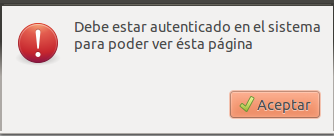
\includegraphics[width=5cm]{Capitulo8InterfacesWeb/Imagenes/Autenticado.png}
	\caption{Alerta sobre usuario no autenticado.}
	\label{fig:estruApp}	
\end{figure}

Posteriormente será direccionado a la página inicial del sitio. En caso de que el usuario no sea administrador e intente ingresar alguna de las páginas donde se realizan modificaciones a la base de datos, se le mostrará el siguiente mensaje:

\begin{figure}[H]
	\centering
	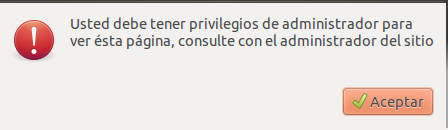
\includegraphics[width=5.5cm]{Capitulo8InterfacesWeb/Imagenes/Administrador.png}
	\caption{Alerta sobre usuario sin rol de administrador.}
	\label{fig:estruApp}	
\end{figure}

Posteriormente será direccionado a la página inicial del sitio.\\\\
Es de anotar que las restricciones están impuestas en lenguaje \textit{PHP} por lo que no es posible infringir estas restricciones deshabilitando el lenguaje \textit{Javascript} en el navegador Web.

